\chapter{Alcances de la Memoria}
\label{alcances}

\section{Problema a resolver}

Actualmente Chile no cuenta con plantas de energía solar fotovoltaica conectadas a sus redes centrales de distribucion (SIC\gloss{SIC}, SING\gloss{SING}, SM\gloss{SM}, SA\gloss{SA}), debido a problemas legales y de normativas tecnicas, la mayoria de las plantas solares que generan energia en chile son plantas aisladas o conectadas a sistemas de distribucion privados, como por ejemplo Calama Solar 3\cite{plantaSolar:1} y Subsole\cite{subsole:2}.

La Red Solar para Latinoamerica y el Caribe(RedSolLac) tiene por objetivo contribuir al desarrollo y aprovechamiento de la energia solar fotovoltaica. Ello mediante una plataforma de difusión de información, que facilita la cooperación y colaboración mutua de instituciones, empresas, profesionales y personas interesadas.
Para apoyar la construccion de de la plataforma de difucion de RedSolLac, Esta ha encargado el desarrollo de una aplicacion informática, que permita exponer de forma gráfica información de producción de energía para plantas solares fotovoltaicas, así como de estaciones de monitoreo meteorológicas, además requiere de una herramienta que le permita calcular costos de producción de energía para apoyar en la toma de desiciones respecto de la construcción de nuevas plantas de energía solar.

\begin{figure}[h!]
        \centering
        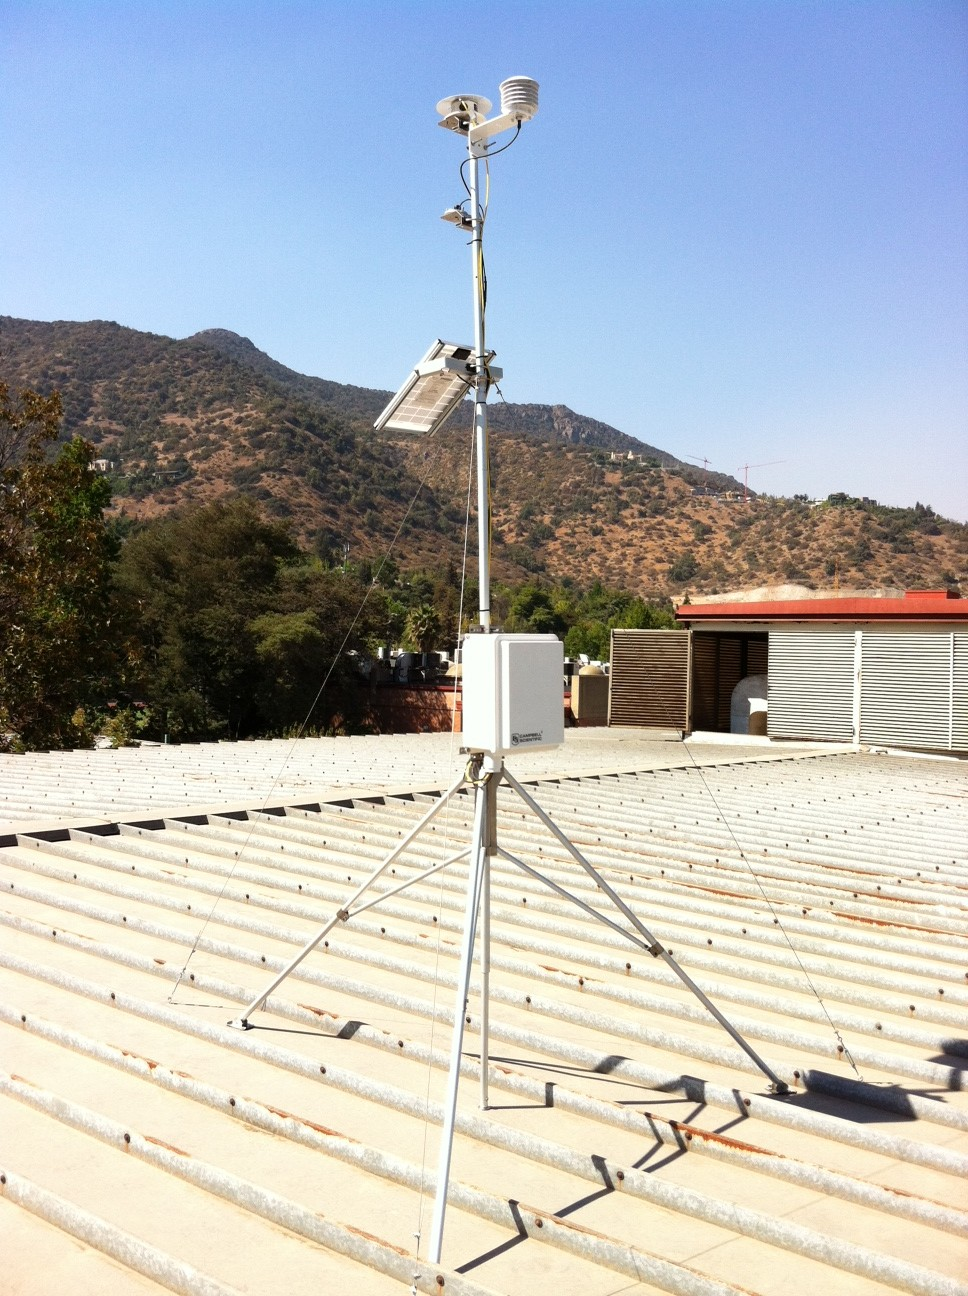
\includegraphics[scale=0.2]{images/estacionMedicionFch}
        \caption{Estación de medición de radiación solar en Fundación Chile, Vitacura - Santiago.}
	\label{fotoEstacionFch}
\end{figure}

(foto planta marcelo mena )

Para el desarrollo de este sistema Fundacion Chile utilizará datos de radiación solar y producción de energia provenientes de diferentes fuentes, tales como, datos de adquisición propia, datos estadisticos publicados por la Comisión Nacional de Energía (\gloss{cne}) y datos de la planta residencial ''MarceloMena''.

Actualmente, RedSolLAC no cuenta con ningun sistema informático que le permita exponer a sus usuarios las lecturas de las estaciones y plantas solares que pertenecen a la red, por lo que es necesario implementar un sistema que permita publicar dicha información.\\

Los datos de adquisición propia provienen de una estación de medición de radiación solar, temperatura y humedad ambiente, instalada en Fundación Chile, en la comuna de Vitacura, Santiago de Chile. Esta estación (Ver. Fig.\ref{fotoEstacionFch}) en conjunto con la planta fotovoltaica (Ver. Fig. \ref{fotoPlantaMarcelo}), proporcionarán la información de radiación solar para la calculadora fotovoltaica y la verificación de cálculos propueststos en esta memoria.\\
Los datos provenientes de la planta ''MarceloMena'' corresponden a una pequeña planta de produccion residencial con el fin de abastecer de energia a un vivienda en la comuna de Vitacura en Santiago de Chile. Estos datos son de especial interes ya que permitiran realizar una comparacion entre los resultados de la simulacion entregados por la ''calculadora'' desarrollada y datos de produccion empirica.

Los principales actores y usuarios de este sistema son todos los miembros de la RedSolLAC, interesados en recibir y compartir información relacionada con la energía solar fotovoltaica. En todo caso la plataforma es abierta por lo que cualquier otro usuario puede acceder a esta información.\\

El BID a través del proyecto RedSolLac que desarrolla la Fundación Chile espera conectar a los actores claves en el desarrollo de la energia solar fotovoltaica de Latinoamérica y el Caribe. En la actualidad, existen pocos actores en la región, por lo que el conocimiento técnico en esta materia se reduce a experiencias de universidades y algunas iniciativas privadas aisladas. RedSolLAC busca convertirse en un sitio de referencia para el estudio y desarrollo de nuevas iniciativas solares.\\

El desarrollo de esta memoria permite a la comunidad de la RedSolLac contar con una gran base de datos para ofrecer a todos sus usuarios, así como diversas aplicaciones en su plataforma para la difunción y el patrocinio de la energía solar en la región. Una red como esta potencia el desarrollo de todas las energías renovables no convencionales (\gloss{ERNC}) especialmente la fotovoltaica, esto se traduce en un beneficio medioambiental directo para toda la comunidad perteneciente a la ''red'' y a la población en general.

\section{Objetivo principal de la solución}
Desarrollar e implementar un sistema informático para la RedSolLAC que permita interconectar equipos y estaciones de medición solar para la recolección y explotación de datos e información técnica.

\section{Objetivos específicos de la solución}
\begin{itemize}
\item Interconectar los diferentes sistemas que componen las estaciones de medición para que exista una comunicación efectiva entre dichos sistemas y una base de datos común en Internet.
\item Desarrollo de un sistema Web capaz de procesar y publicar la información recopilada de una planta de energía solar.
\item Desarrollo de una calculadora online para sistemas fotovoltaicos, que permita dimensionar y estimar los costos de produccion de energia electrica.
\item Realizar pruebas de la plataforma en conjunto con todos sus componentes, comparar los datos obtenidos con datos recopilados de otras fuentes. Estas prubas permitiran validar el funcionamiento del software asi como la acertividad del metodo de calculo y estimacion electrica implementado en la solución.
\end{itemize}

\section{Requerimientos del sistema}
Para el desarrollo del sistema planteado, el BID, RedSolLAC y Fundacion Chile han establecido una serie de requerimientos de diferente naturaleza los cuales se detallan en los proximos capitulos (Ver Figs. \ref{tablaFuncional} y \ref{tablaNoFuncional}), ademas la figura \ref{fig:demanda} se presenta como una idea de presentacion de datos originados por las estaciones y que deben ser presentadas de forma interactiva en el sitio Web de RedSolLAC.

\begin{figure}[h!]
        \centering
        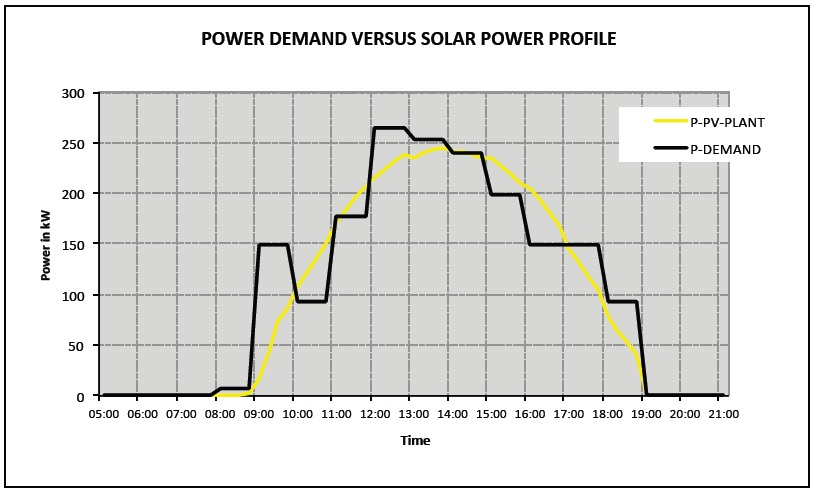
\includegraphics[scale=0.5]{images/demandaGeneracionSubSole}
        \caption{Gráfico de ejemplo de la curva de generación de energía solar.}
	\label{fig:demanda}
\end{figure}

\subsection{Requerimientos funcionales}
\begin{table}[h!]
\caption{Tabla de requerimientos funcionales}
\label{tablaFuncional}
\begin{tabular}{| c | p{11cm} |}
	\hline
	\textbf{Requerimiento}	&	\textbf{Detalle}	\\
	\hline
	RF-1	&	Registro de datos en linea, las estaciones deben ser programadas para registrar los datos capturados en una base de datos externa en internet, el regisstro de datos debe ser cada 1 minuto.	\\
	\hline
	RF-2	&	La aplicacion debe ser capas de visualizar datos actuales historicos e instantaneos, se debe prporcionar un modulo de visualizacion de datos que permita al usuario visualizar de manera total o parcial los datos registrados por las estaciones, permitiendo seleccionar periodos de tiempo y diferentes tipos de datos proporcionados por los diferentes sensores que conforman la estacion(ver Fig:\ref{fig:demanda}). 	\\
	\hline
	RF-3	&	Descarga de datos, los datos registrados por las estaciones deben estar disponibles para su descarga en un formato practico para la utilizacion de estos por usuarios expertos, pudiendo estos usuarios descargar datos de acuerdo a un periodo de tiempo especificado.	\\
	\hline
	RF-4	&	Permitir el ingreso de informacion, la aplicacion debe permitir el ingreso de parametros geograficos, informacion tecnica de planta y datos economicos para realizar los calculos del dimencionamiento de una planta de energia solar 	\\
delo de radiación solar para  conversion de datos sinteticos de radiacion solar en valores horarios''
	\hline
	RF-5	&	Implementar un modelo de calculo de energia horario basado en el documento ''Modelo de radiación solar para conversion de datos sinteticos de radiacion solar en valores horarios'', extracto de la memoria de ''master'' ''Dimensionamiento para sistemas solar termicos en la republica de Chile\ref{memoriaEdu}'' (Ver anexo \ref{memoriaEdu2})\\
	\hline
	RF-6	&	Calcular y exponer resultados de produccion energetica, los resultados deben ser verificables y comparables con otros sistemas, los calculos deben presentar errores no superiroes al 5\%	\\
	\hline
\end{tabular}
\end{table}

\subsection{requerimientos no funcionales}
\begin{table}[h!]
\caption{Tabla de requerimientos no funcionales}
\label{tablaNoFuncional}
\begin{tabular}{| c | p{11cm} |}
	\hline
	\textbf{Requerimiento}	&	\textbf{Detalle}	\\
	\hline
	RNF-1	&	La aplicacion debe ser independiente del Sistema operativo y del navegador utilizado por el usuarios final	\\
	\hline
	RNF-2	&	Es necesario que la aplicacion se integre con la imagen coorporativa de la RedSolLac	\\
	\hline
	RNF-3	&	El sistema debe entregar estabilidad y muy alta confiabilidad en el registro y amacenamiento de datos	\\
	\hline
	RNF-4	&	La aplicacion debe ser portable y facilmente adaptable para funcionar con multiples fuentes de datos 	\\
	\hline
	RNF-5	&	La aplicacion debe proporcionar un minimo estandar de seguridad que permita asegurar la confiabilidad de los datos	\\
	\hline
	RNF-6	&	La aplicacion debe entregar un resultado al usuario final en tiempo aceptable no mayor a 5 seg	\\
	\hline
\end{tabular}
\end{table}


